\documentclass[journal,12pt,twocolumn]{IEEEtran}
\usepackage[utf8]{inputenc}
\usepackage{amssymb,amsmath,mathtools} 
\usepackage{amsfonts}  
\usepackage{graphicx}  
\usepackage{times}
\graphicspath{{images/}}
\DeclareGraphicsExtensions{.pdf,.eps,.ps,.png,.jpg,.jpeg}
\newcommand{\C}{\circ}
\title{\textbf{AI1110 Assignment 1}
\author{AI21BTECH11001 }}
\date{March 2022}

\begin{document}

\maketitle
\begin{center}
{ICSE Grade 10 2014 paper}\end{center}

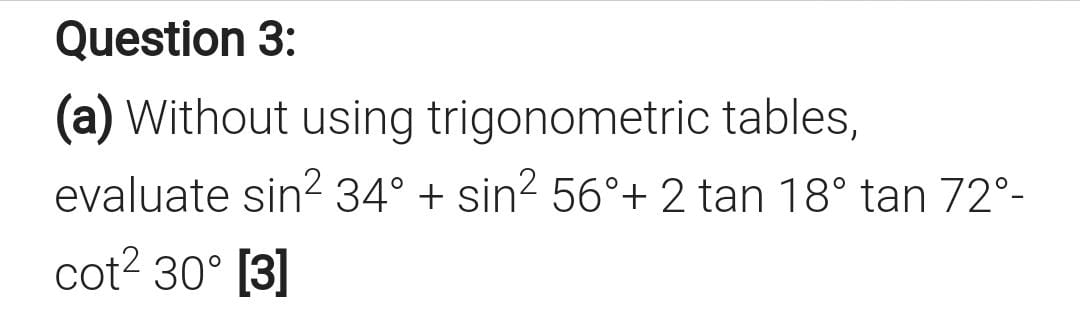
\includegraphics[scale=0.22]{main.jpeg}

\textbf{Solution:}
$$
    sin^2 34^\C + sin^2 56^\C +
 2tan 18^\C tan 72^\C - cot^2 30^\C 
$$


$$sin^2 34^\C + sin^2(90^\C - 34^\C)+2tan18^\C tan(90^\C- 18^\C) $$
$$- cot^2 30^\C$$

$$sin^2 34^\C + cos^2 34^\C +2tan18^\C cot18^\C - cot^2 30^\C $$

$$ 1 + 2tan18 ^\C \frac{1}{tan18^\C} - (\sqrt{3})^2$$

$$1 + 2 - 3$$
$$ 0$$
\end{document}
